% Options for packages loaded elsewhere
\PassOptionsToPackage{unicode}{hyperref}
\PassOptionsToPackage{hyphens}{url}
%
\documentclass[
]{article}
\usepackage{amsmath,amssymb}
\usepackage{iftex}
\ifPDFTeX
  \usepackage[T1]{fontenc}
  \usepackage[utf8]{inputenc}
  \usepackage{textcomp} % provide euro and other symbols
\else % if luatex or xetex
  \usepackage{unicode-math} % this also loads fontspec
  \defaultfontfeatures{Scale=MatchLowercase}
  \defaultfontfeatures[\rmfamily]{Ligatures=TeX,Scale=1}
\fi
\usepackage{lmodern}
\ifPDFTeX\else
  % xetex/luatex font selection
\fi
% Use upquote if available, for straight quotes in verbatim environments
\IfFileExists{upquote.sty}{\usepackage{upquote}}{}
\IfFileExists{microtype.sty}{% use microtype if available
  \usepackage[]{microtype}
  \UseMicrotypeSet[protrusion]{basicmath} % disable protrusion for tt fonts
}{}
\makeatletter
\@ifundefined{KOMAClassName}{% if non-KOMA class
  \IfFileExists{parskip.sty}{%
    \usepackage{parskip}
  }{% else
    \setlength{\parindent}{0pt}
    \setlength{\parskip}{6pt plus 2pt minus 1pt}}
}{% if KOMA class
  \KOMAoptions{parskip=half}}
\makeatother
\usepackage{xcolor}
\usepackage[margin=1in]{geometry}
\usepackage{color}
\usepackage{fancyvrb}
\newcommand{\VerbBar}{|}
\newcommand{\VERB}{\Verb[commandchars=\\\{\}]}
\DefineVerbatimEnvironment{Highlighting}{Verbatim}{commandchars=\\\{\}}
% Add ',fontsize=\small' for more characters per line
\usepackage{framed}
\definecolor{shadecolor}{RGB}{248,248,248}
\newenvironment{Shaded}{\begin{snugshade}}{\end{snugshade}}
\newcommand{\AlertTok}[1]{\textcolor[rgb]{0.94,0.16,0.16}{#1}}
\newcommand{\AnnotationTok}[1]{\textcolor[rgb]{0.56,0.35,0.01}{\textbf{\textit{#1}}}}
\newcommand{\AttributeTok}[1]{\textcolor[rgb]{0.13,0.29,0.53}{#1}}
\newcommand{\BaseNTok}[1]{\textcolor[rgb]{0.00,0.00,0.81}{#1}}
\newcommand{\BuiltInTok}[1]{#1}
\newcommand{\CharTok}[1]{\textcolor[rgb]{0.31,0.60,0.02}{#1}}
\newcommand{\CommentTok}[1]{\textcolor[rgb]{0.56,0.35,0.01}{\textit{#1}}}
\newcommand{\CommentVarTok}[1]{\textcolor[rgb]{0.56,0.35,0.01}{\textbf{\textit{#1}}}}
\newcommand{\ConstantTok}[1]{\textcolor[rgb]{0.56,0.35,0.01}{#1}}
\newcommand{\ControlFlowTok}[1]{\textcolor[rgb]{0.13,0.29,0.53}{\textbf{#1}}}
\newcommand{\DataTypeTok}[1]{\textcolor[rgb]{0.13,0.29,0.53}{#1}}
\newcommand{\DecValTok}[1]{\textcolor[rgb]{0.00,0.00,0.81}{#1}}
\newcommand{\DocumentationTok}[1]{\textcolor[rgb]{0.56,0.35,0.01}{\textbf{\textit{#1}}}}
\newcommand{\ErrorTok}[1]{\textcolor[rgb]{0.64,0.00,0.00}{\textbf{#1}}}
\newcommand{\ExtensionTok}[1]{#1}
\newcommand{\FloatTok}[1]{\textcolor[rgb]{0.00,0.00,0.81}{#1}}
\newcommand{\FunctionTok}[1]{\textcolor[rgb]{0.13,0.29,0.53}{\textbf{#1}}}
\newcommand{\ImportTok}[1]{#1}
\newcommand{\InformationTok}[1]{\textcolor[rgb]{0.56,0.35,0.01}{\textbf{\textit{#1}}}}
\newcommand{\KeywordTok}[1]{\textcolor[rgb]{0.13,0.29,0.53}{\textbf{#1}}}
\newcommand{\NormalTok}[1]{#1}
\newcommand{\OperatorTok}[1]{\textcolor[rgb]{0.81,0.36,0.00}{\textbf{#1}}}
\newcommand{\OtherTok}[1]{\textcolor[rgb]{0.56,0.35,0.01}{#1}}
\newcommand{\PreprocessorTok}[1]{\textcolor[rgb]{0.56,0.35,0.01}{\textit{#1}}}
\newcommand{\RegionMarkerTok}[1]{#1}
\newcommand{\SpecialCharTok}[1]{\textcolor[rgb]{0.81,0.36,0.00}{\textbf{#1}}}
\newcommand{\SpecialStringTok}[1]{\textcolor[rgb]{0.31,0.60,0.02}{#1}}
\newcommand{\StringTok}[1]{\textcolor[rgb]{0.31,0.60,0.02}{#1}}
\newcommand{\VariableTok}[1]{\textcolor[rgb]{0.00,0.00,0.00}{#1}}
\newcommand{\VerbatimStringTok}[1]{\textcolor[rgb]{0.31,0.60,0.02}{#1}}
\newcommand{\WarningTok}[1]{\textcolor[rgb]{0.56,0.35,0.01}{\textbf{\textit{#1}}}}
\usepackage{graphicx}
\makeatletter
\def\maxwidth{\ifdim\Gin@nat@width>\linewidth\linewidth\else\Gin@nat@width\fi}
\def\maxheight{\ifdim\Gin@nat@height>\textheight\textheight\else\Gin@nat@height\fi}
\makeatother
% Scale images if necessary, so that they will not overflow the page
% margins by default, and it is still possible to overwrite the defaults
% using explicit options in \includegraphics[width, height, ...]{}
\setkeys{Gin}{width=\maxwidth,height=\maxheight,keepaspectratio}
% Set default figure placement to htbp
\makeatletter
\def\fps@figure{htbp}
\makeatother
\setlength{\emergencystretch}{3em} % prevent overfull lines
\providecommand{\tightlist}{%
  \setlength{\itemsep}{0pt}\setlength{\parskip}{0pt}}
\setcounter{secnumdepth}{-\maxdimen} % remove section numbering
\ifLuaTeX
  \usepackage{selnolig}  % disable illegal ligatures
\fi
\usepackage{bookmark}
\IfFileExists{xurl.sty}{\usepackage{xurl}}{} % add URL line breaks if available
\urlstyle{same}
\hypersetup{
  pdftitle={Lab1\_notes},
  hidelinks,
  pdfcreator={LaTeX via pandoc}}

\title{Lab1\_notes}
\author{}
\date{\vspace{-2.5em}2024-09-04}

\begin{document}
\maketitle

\subsection{Sample code}\label{sample-code}

\begin{Shaded}
\begin{Highlighting}[]
\CommentTok{\# Load libraries.}
\DocumentationTok{\#\# install via \textasciigrave{}install.packages("name")\textasciigrave{}}
\FunctionTok{library}\NormalTok{(ggplot2)}
\FunctionTok{library}\NormalTok{(maps)}
\FunctionTok{library}\NormalTok{(tidyverse)}
\end{Highlighting}
\end{Shaded}

\begin{verbatim}
## -- Attaching core tidyverse packages ------------------------ tidyverse 2.0.0 --
## v dplyr     1.1.3     v readr     2.1.4
## v forcats   1.0.0     v stringr   1.5.0
## v lubridate 1.9.2     v tibble    3.2.1
## v purrr     1.0.2     v tidyr     1.3.0
## -- Conflicts ------------------------------------------ tidyverse_conflicts() --
## x dplyr::filter() masks stats::filter()
## x dplyr::lag()    masks stats::lag()
## x purrr::map()    masks maps::map()
## i Use the conflicted package (<http://conflicted.r-lib.org/>) to force all conflicts to become errors
\end{verbatim}

\begin{Shaded}
\begin{Highlighting}[]
\CommentTok{\# Read presidential popular vote. }
\NormalTok{d\_popvote }\OtherTok{\textless{}{-}} \FunctionTok{read\_csv}\NormalTok{(}\StringTok{"popvote\_1948{-}2020.csv"}\NormalTok{)}
\end{Highlighting}
\end{Shaded}

\begin{verbatim}
## Rows: 38 Columns: 9
## -- Column specification --------------------------------------------------------
## Delimiter: ","
## chr (2): party, candidate
## dbl (3): year, pv, pv2p
## lgl (4): winner, incumbent, incumbent_party, prev_admin
## 
## i Use `spec()` to retrieve the full column specification for this data.
## i Specify the column types or set `show_col_types = FALSE` to quiet this message.
\end{verbatim}

\begin{Shaded}
\begin{Highlighting}[]
\CommentTok{\# Subset data to most recent past election year. }
\NormalTok{d\_popvote }\SpecialCharTok{|\textgreater{}} 
  \FunctionTok{filter}\NormalTok{(year }\SpecialCharTok{==} \DecValTok{2020}\NormalTok{) }\SpecialCharTok{|\textgreater{}} 
  \FunctionTok{select}\NormalTok{(party, candidate, pv2p)}
\end{Highlighting}
\end{Shaded}

\begin{verbatim}
## # A tibble: 2 x 3
##   party      candidate         pv2p
##   <chr>      <chr>            <dbl>
## 1 democrat   Biden, Joseph R.  52.3
## 2 republican Trump, Donald J.  47.7
\end{verbatim}

\begin{Shaded}
\begin{Highlighting}[]
\CommentTok{\# Pivot data to wide format with party names as columns and two{-}party vote share as values.}
\NormalTok{(d\_popvote\_wide }\OtherTok{\textless{}{-}}\NormalTok{ d\_popvote }\SpecialCharTok{|\textgreater{}}
    \FunctionTok{select}\NormalTok{(year, party, pv2p) }\SpecialCharTok{|\textgreater{}}
    \FunctionTok{pivot\_wider}\NormalTok{(}\AttributeTok{names\_from =}\NormalTok{ party, }\AttributeTok{values\_from =}\NormalTok{ pv2p))}
\end{Highlighting}
\end{Shaded}

\begin{verbatim}
## # A tibble: 19 x 3
##     year democrat republican
##    <dbl>    <dbl>      <dbl>
##  1  1948     52.3       47.7
##  2  1952     44.7       55.3
##  3  1956     42.2       57.8
##  4  1960     50.1       49.9
##  5  1964     61.3       38.7
##  6  1968     49.6       50.4
##  7  1972     38.2       61.8
##  8  1976     51.1       48.9
##  9  1980     44.8       55.2
## 10  1984     40.9       59.1
## 11  1988     46.2       53.8
## 12  1992     53.6       46.4
## 13  1996     54.8       45.2
## 14  2000     50.3       49.7
## 15  2004     48.7       51.3
## 16  2008     53.8       46.2
## 17  2012     51.9       48.1
## 18  2016     51.2       48.8
## 19  2020     52.3       47.7
\end{verbatim}

\begin{Shaded}
\begin{Highlighting}[]
\CommentTok{\# Modify winner column to show "D" if Democrats win and "R" if Republicans win. }
\NormalTok{(d\_popvote\_wide }\OtherTok{\textless{}{-}}\NormalTok{ d\_popvote\_wide }\SpecialCharTok{|\textgreater{}} 
    \FunctionTok{mutate}\NormalTok{(}\AttributeTok{winner =} \FunctionTok{case\_when}\NormalTok{(democrat }\SpecialCharTok{\textgreater{}}\NormalTok{ republican }\SpecialCharTok{\textasciitilde{}} \StringTok{"D"}\NormalTok{,}
                              \ConstantTok{TRUE} \SpecialCharTok{\textasciitilde{}} \StringTok{"R"}\NormalTok{)))}
\end{Highlighting}
\end{Shaded}

\begin{verbatim}
## # A tibble: 19 x 4
##     year democrat republican winner
##    <dbl>    <dbl>      <dbl> <chr> 
##  1  1948     52.3       47.7 D     
##  2  1952     44.7       55.3 R     
##  3  1956     42.2       57.8 R     
##  4  1960     50.1       49.9 D     
##  5  1964     61.3       38.7 D     
##  6  1968     49.6       50.4 R     
##  7  1972     38.2       61.8 R     
##  8  1976     51.1       48.9 D     
##  9  1980     44.8       55.2 R     
## 10  1984     40.9       59.1 R     
## 11  1988     46.2       53.8 R     
## 12  1992     53.6       46.4 D     
## 13  1996     54.8       45.2 D     
## 14  2000     50.3       49.7 D     
## 15  2004     48.7       51.3 R     
## 16  2008     53.8       46.2 D     
## 17  2012     51.9       48.1 D     
## 18  2016     51.2       48.8 D     
## 19  2020     52.3       47.7 D
\end{verbatim}

\begin{Shaded}
\begin{Highlighting}[]
\CommentTok{\# Summarize data with respect to winners. }
\NormalTok{d\_popvote\_wide }\SpecialCharTok{|\textgreater{}} 
  \FunctionTok{group\_by}\NormalTok{(winner) }\SpecialCharTok{|\textgreater{}}
  \FunctionTok{summarise}\NormalTok{(}\AttributeTok{races =} \FunctionTok{n}\NormalTok{())}
\end{Highlighting}
\end{Shaded}

\begin{verbatim}
## # A tibble: 2 x 2
##   winner races
##   <chr>  <int>
## 1 D         11
## 2 R          8
\end{verbatim}

\begin{Shaded}
\begin{Highlighting}[]
\DocumentationTok{\#\#\#\#{-}{-}{-}{-}{-}{-}{-}{-}{-}{-}{-}{-}{-}{-}{-}{-}{-}{-}{-}{-}{-}{-}{-}{-}{-}{-}{-}{-}{-}{-}{-}{-}{-}{-}{-}{-}{-}{-}{-}{-}{-}{-}{-}{-}{-}{-}{-}{-}{-}{-}{-}{-}{-}{-}{-}{-}{-}{-}\#}
\DocumentationTok{\#\#\#\# Visualize trends in national presidential popular vote. }
\DocumentationTok{\#\#\#\#{-}{-}{-}{-}{-}{-}{-}{-}{-}{-}{-}{-}{-}{-}{-}{-}{-}{-}{-}{-}{-}{-}{-}{-}{-}{-}{-}{-}{-}{-}{-}{-}{-}{-}{-}{-}{-}{-}{-}{-}{-}{-}{-}{-}{-}{-}{-}{-}{-}{-}{-}{-}{-}{-}{-}{-}{-}{-}\#}

\CommentTok{\# Visualize the two{-}party presidential popular over time. }
\NormalTok{d\_popvote\_plot }\OtherTok{\textless{}{-}} \FunctionTok{ggplot}\NormalTok{(}\AttributeTok{data =}\NormalTok{ d\_popvote,}
                         \AttributeTok{mapping =} \FunctionTok{aes}\NormalTok{(}\AttributeTok{x =}\NormalTok{ year, }\AttributeTok{y =}\NormalTok{ pv2p, }\AttributeTok{color =}\NormalTok{ party)) }\SpecialCharTok{+} 
  \FunctionTok{geom\_line}\NormalTok{() }\SpecialCharTok{+}
  \FunctionTok{scale\_color\_manual}\NormalTok{(}\AttributeTok{values =} \FunctionTok{c}\NormalTok{(}\StringTok{"dodgerblue"}\NormalTok{, }\StringTok{"firebrick"}\NormalTok{)) }\SpecialCharTok{+}
  \FunctionTok{theme\_bw}\NormalTok{() }\SpecialCharTok{+}
  \FunctionTok{labs}\NormalTok{(}\AttributeTok{x =} \StringTok{"Year"}\NormalTok{,}
       \AttributeTok{y =} \StringTok{"Percent of Two{-}Party Voteshare"}\NormalTok{,}
       \AttributeTok{title =} \StringTok{"Two{-}Party Presidential Popular Voteshare Over Time"}\NormalTok{)}

\NormalTok{d\_popvote\_plot}
\end{Highlighting}
\end{Shaded}

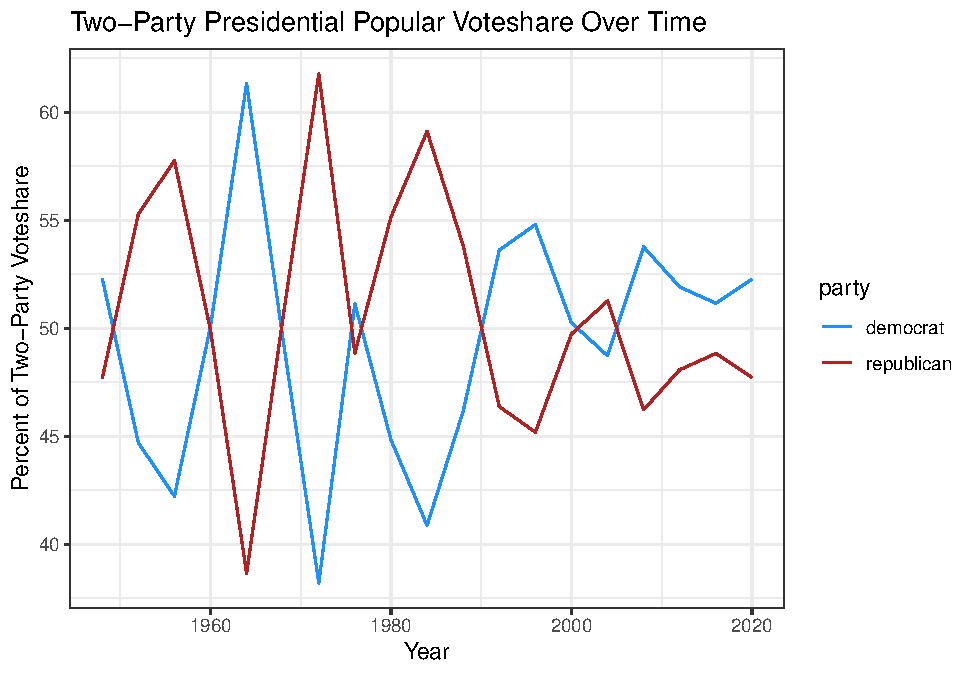
\includegraphics{Lab1-notes_files/figure-latex/unnamed-chunk-1-1.pdf}

\begin{Shaded}
\begin{Highlighting}[]
\DocumentationTok{\#\#\#\#{-}{-}{-}{-}{-}{-}{-}{-}{-}{-}{-}{-}{-}{-}{-}{-}{-}{-}{-}{-}{-}{-}{-}{-}{-}{-}{-}{-}{-}{-}{-}{-}{-}{-}{-}{-}{-}{-}{-}{-}{-}{-}{-}{-}{-}{-}{-}{-}{-}{-}{-}{-}{-}{-}{-}{-}{-}{-}\#}
\DocumentationTok{\#\#\#\# State{-}by{-}state map of presidential popular votes.}
\DocumentationTok{\#\#\#\#{-}{-}{-}{-}{-}{-}{-}{-}{-}{-}{-}{-}{-}{-}{-}{-}{-}{-}{-}{-}{-}{-}{-}{-}{-}{-}{-}{-}{-}{-}{-}{-}{-}{-}{-}{-}{-}{-}{-}{-}{-}{-}{-}{-}{-}{-}{-}{-}{-}{-}{-}{-}{-}{-}{-}{-}{-}{-}\#}

\CommentTok{\# Sequester shapefile of states from \textasciigrave{}maps\textasciigrave{} library.}
\NormalTok{states\_map }\OtherTok{\textless{}{-}} \FunctionTok{map\_data}\NormalTok{(}\StringTok{"state"}\NormalTok{)}

\CommentTok{\# Read wide version of dataset that can be used to compare candidate votes with one another. }
\NormalTok{d\_pvstate\_wide }\OtherTok{\textless{}{-}} \FunctionTok{read\_csv}\NormalTok{(}\StringTok{"clean\_wide\_state\_2pv\_1948\_2020.csv"}\NormalTok{)}
\end{Highlighting}
\end{Shaded}

\begin{verbatim}
## Rows: 959 Columns: 14
## -- Column specification --------------------------------------------------------
## Delimiter: ","
## chr  (1): state
## dbl (13): year, D_pv, R_pv, D_pv2p, R_pv2p, D_pv_lag1, R_pv_lag1, D_pv2p_lag...
## 
## i Use `spec()` to retrieve the full column specification for this data.
## i Specify the column types or set `show_col_types = FALSE` to quiet this message.
\end{verbatim}

\begin{Shaded}
\begin{Highlighting}[]
\CommentTok{\# Merge d\_pvstate\_wide with state\_map.}
\NormalTok{d\_pvstate\_wide}\SpecialCharTok{$}\NormalTok{region }\OtherTok{\textless{}{-}} \FunctionTok{tolower}\NormalTok{(d\_pvstate\_wide}\SpecialCharTok{$}\NormalTok{state)}

\NormalTok{pv\_map }\OtherTok{\textless{}{-}}\NormalTok{ d\_pvstate\_wide }\SpecialCharTok{|\textgreater{}}
  \FunctionTok{filter}\NormalTok{(year }\SpecialCharTok{==} \DecValTok{2020}\NormalTok{) }\SpecialCharTok{|\textgreater{}}
  \FunctionTok{left\_join}\NormalTok{(states\_map, }\AttributeTok{by =} \StringTok{"region"}\NormalTok{)}
\end{Highlighting}
\end{Shaded}

\begin{Shaded}
\begin{Highlighting}[]
\CommentTok{\# Make map grid of state winners for each election year available in the dataset.}
\NormalTok{pv\_map }\OtherTok{\textless{}{-}}\NormalTok{ d\_pvstate\_wide }\SpecialCharTok{|\textgreater{}}
  \FunctionTok{filter}\NormalTok{(year }\SpecialCharTok{==} \DecValTok{2020}\NormalTok{) }\SpecialCharTok{|\textgreater{}}
  \FunctionTok{left\_join}\NormalTok{(states\_map, }\AttributeTok{by =} \StringTok{"region"}\NormalTok{)}

\NormalTok{pv\_win\_map }\OtherTok{\textless{}{-}}\NormalTok{ pv\_map }\SpecialCharTok{|\textgreater{}}
  \FunctionTok{mutate}\NormalTok{(}\AttributeTok{winner =} \FunctionTok{if\_else}\NormalTok{(R\_pv2p }\SpecialCharTok{\textgreater{}}\NormalTok{ D\_pv2p, }\StringTok{"republican"}\NormalTok{, }\StringTok{"democrat"}\NormalTok{))}

\NormalTok{pv\_win\_map }\SpecialCharTok{|\textgreater{}}
  \FunctionTok{ggplot}\NormalTok{(}\FunctionTok{aes}\NormalTok{(long, lat, }\AttributeTok{group =}\NormalTok{ group)) }\SpecialCharTok{+}
  \FunctionTok{geom\_polygon}\NormalTok{(}\FunctionTok{aes}\NormalTok{(}\AttributeTok{fill =}\NormalTok{ winner)) }\SpecialCharTok{+}
  \FunctionTok{scale\_fill\_manual}\NormalTok{(}\AttributeTok{values =} \FunctionTok{c}\NormalTok{(}\StringTok{"dodgerblue"}\NormalTok{, }\StringTok{"firebrick"}\NormalTok{)) }\SpecialCharTok{+}
  \FunctionTok{theme\_void}\NormalTok{()}
\end{Highlighting}
\end{Shaded}

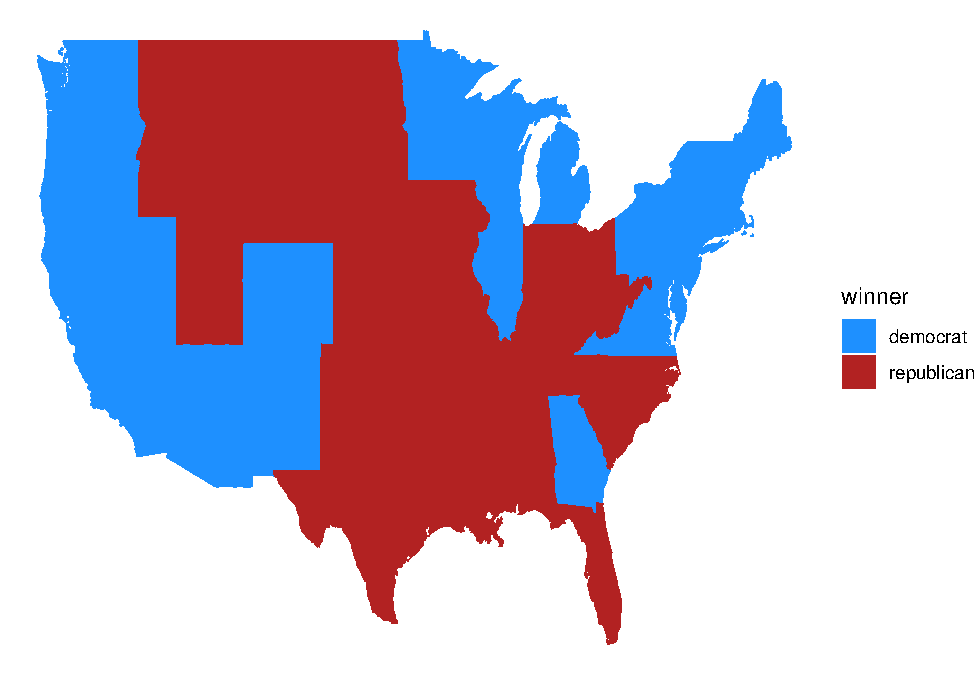
\includegraphics{Lab1-notes_files/figure-latex/unnamed-chunk-2-1.pdf}

\begin{Shaded}
\begin{Highlighting}[]
\NormalTok{d\_pvstate\_wide }\SpecialCharTok{|\textgreater{}}
  \FunctionTok{filter}\NormalTok{(year }\SpecialCharTok{\textgreater{}=} \DecValTok{1980}\NormalTok{) }\SpecialCharTok{|\textgreater{}}
  \FunctionTok{left\_join}\NormalTok{(states\_map, }\AttributeTok{by =} \StringTok{"region"}\NormalTok{) }\SpecialCharTok{|\textgreater{}}
  \FunctionTok{mutate}\NormalTok{(}\AttributeTok{winner =} \FunctionTok{if\_else}\NormalTok{(R\_pv2p }\SpecialCharTok{\textgreater{}}\NormalTok{ D\_pv2p, }\StringTok{"republican"}\NormalTok{, }\StringTok{"democrat"}\NormalTok{)) }\SpecialCharTok{|\textgreater{}}
  \FunctionTok{ggplot}\NormalTok{(}\FunctionTok{aes}\NormalTok{(long, lat, }\AttributeTok{group =}\NormalTok{ group)) }\SpecialCharTok{+}
  \FunctionTok{facet\_wrap}\NormalTok{(}\AttributeTok{facets =}\NormalTok{ year }\SpecialCharTok{\textasciitilde{}}\NormalTok{.) }\SpecialCharTok{+}
  \FunctionTok{geom\_polygon}\NormalTok{(}\FunctionTok{aes}\NormalTok{(}\AttributeTok{fill =}\NormalTok{ winner), }\AttributeTok{color =} \StringTok{"white"}\NormalTok{) }\SpecialCharTok{+}
  \FunctionTok{scale\_fill\_manual}\NormalTok{(}\AttributeTok{values =} \FunctionTok{c}\NormalTok{(}\StringTok{"dodgerblue"}\NormalTok{, }\StringTok{"firebrick"}\NormalTok{)) }\SpecialCharTok{+}
  \FunctionTok{theme\_void}\NormalTok{() }\SpecialCharTok{+}
    \FunctionTok{ggtitle}\NormalTok{(}\StringTok{"Presidential Vote Share (1980 {-} 2020)"}\NormalTok{)}
\end{Highlighting}
\end{Shaded}

\begin{verbatim}
## Warning in left_join(filter(d_pvstate_wide, year >= 1980), states_map, by = "region"): Detected an unexpected many-to-many relationship between `x` and `y`.
## i Row 1 of `x` matches multiple rows in `y`.
## i Row 1 of `y` matches multiple rows in `x`.
## i If a many-to-many relationship is expected, set `relationship =
##   "many-to-many"` to silence this warning.
\end{verbatim}

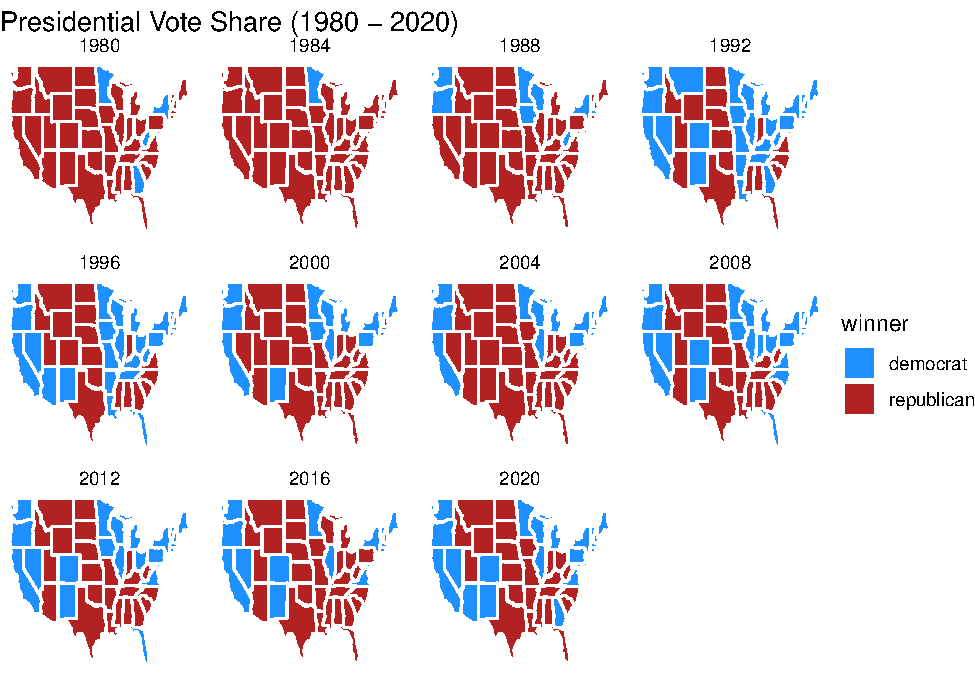
\includegraphics{Lab1-notes_files/figure-latex/unnamed-chunk-2-2.pdf}

\#\#\#\#----------------------------------------------------------\#
\#\#\#\# Forecast: simplified electoral cycle model.
\#\#\#\#----------------------------------------------------------\#

\section{Create prediction (pv2p and margin) based on simplified
electoral cycle
model:}\label{create-prediction-pv2p-and-margin-based-on-simplified-electoral-cycle-model}

\section{\texorpdfstring{vote\_2024 = 3/4\emph{vote\_2020 +
1/4}vote\_2016 (lag1, lag2,
respectively).}{vote\_2024 = 3/4vote\_2020 + 1/4vote\_2016 (lag1, lag2, respectively).}}\label{vote_2024-34vote_2020-14vote_2016-lag1-lag2-respectively.}

\begin{Shaded}
\begin{Highlighting}[]
\CommentTok{\# Plot the margin of victory in a U.S. state map.}

\NormalTok{pv2p\_2024\_states }\OtherTok{\textless{}{-}}\NormalTok{ d\_pvstate\_wide }\SpecialCharTok{|\textgreater{}}
  \FunctionTok{filter}\NormalTok{(year }\SpecialCharTok{==} \DecValTok{2020}\NormalTok{) }\SpecialCharTok{|\textgreater{}}
  \FunctionTok{group\_by}\NormalTok{(state) }\SpecialCharTok{|\textgreater{}}
  \FunctionTok{summarize}\NormalTok{(}\AttributeTok{R\_pv2p\_2024 =} \FloatTok{0.75}\SpecialCharTok{*}\NormalTok{R\_pv2p }\SpecialCharTok{+} \FloatTok{0.25}\SpecialCharTok{*}\NormalTok{R\_pv2p\_lag1,}
            \AttributeTok{D\_pv2p\_2024 =} \FloatTok{0.75}\SpecialCharTok{*}\NormalTok{D\_pv2p }\SpecialCharTok{+} \FloatTok{0.25}\SpecialCharTok{*}\NormalTok{D\_pv2p\_lag1) }\SpecialCharTok{|\textgreater{}}
  \FunctionTok{mutate}\NormalTok{(}\AttributeTok{pv2p\_2024\_margin =}\NormalTok{ R\_pv2p\_2024 }\SpecialCharTok{{-}}\NormalTok{ D\_pv2p\_2024,}
         \AttributeTok{winner =} \FunctionTok{ifelse}\NormalTok{(R\_pv2p\_2024 }\SpecialCharTok{\textgreater{}}\NormalTok{ D\_pv2p\_2024, }\StringTok{"R"}\NormalTok{, }\StringTok{"D"}\NormalTok{),}
         \AttributeTok{region =} \FunctionTok{tolower}\NormalTok{(state))}

\NormalTok{pv2p\_2024\_states }\SpecialCharTok{|\textgreater{}}
  \FunctionTok{left\_join}\NormalTok{(states\_map, }\AttributeTok{by =} \StringTok{"region"}\NormalTok{) }\SpecialCharTok{|\textgreater{}}
  \FunctionTok{ggplot}\NormalTok{(}\FunctionTok{aes}\NormalTok{(long, lat, }\AttributeTok{group =}\NormalTok{ group)) }\SpecialCharTok{+}
  \FunctionTok{geom\_polygon}\NormalTok{(}\FunctionTok{aes}\NormalTok{(}\AttributeTok{fill =}\NormalTok{ pv2p\_2024\_margin), }\AttributeTok{color =} \StringTok{"black"}\NormalTok{) }\SpecialCharTok{+}
  \FunctionTok{scale\_fill\_gradient2}\NormalTok{(}\AttributeTok{high =} \StringTok{"firebrick"}\NormalTok{,}
                      \AttributeTok{low =} \StringTok{"dodgerblue"}\NormalTok{,}
                      \AttributeTok{mid =} \StringTok{"white"}\NormalTok{,}
                      \AttributeTok{name =} \StringTok{"win margin"}\NormalTok{,}
                      \AttributeTok{breaks =} \FunctionTok{c}\NormalTok{(}\SpecialCharTok{{-}}\DecValTok{50}\NormalTok{, }\SpecialCharTok{{-}}\DecValTok{25}\NormalTok{, }\DecValTok{0}\NormalTok{, }\DecValTok{25}\NormalTok{, }\DecValTok{50}\NormalTok{),}
                      \AttributeTok{limits =} \FunctionTok{c}\NormalTok{(}\SpecialCharTok{{-}}\DecValTok{50}\NormalTok{, }\DecValTok{50}\NormalTok{)) }\SpecialCharTok{+}
  \FunctionTok{theme\_void}\NormalTok{()}
\end{Highlighting}
\end{Shaded}

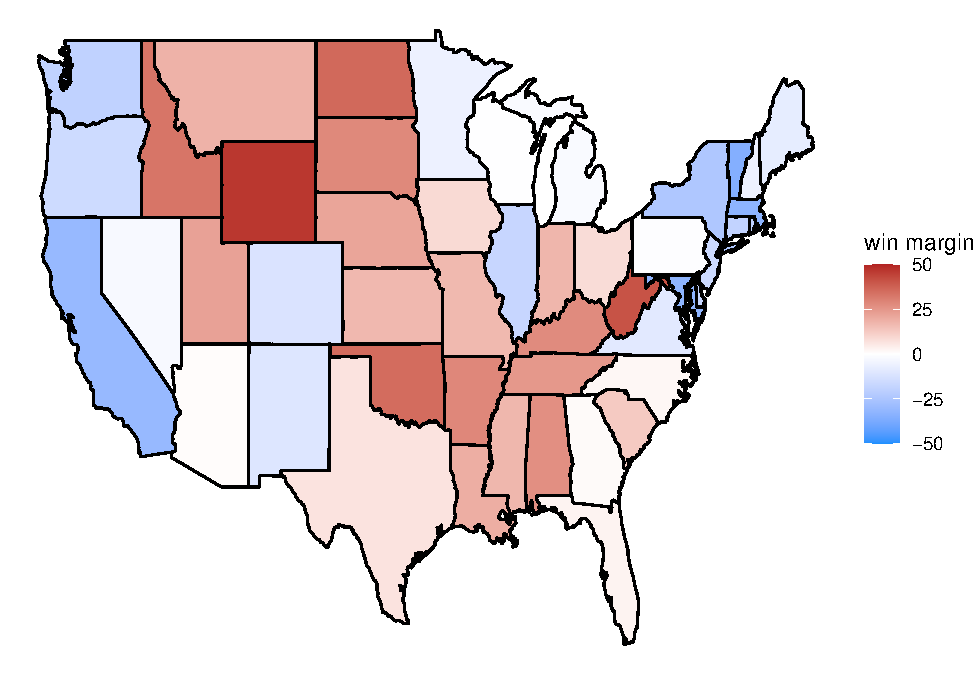
\includegraphics{Lab1-notes_files/figure-latex/unnamed-chunk-3-1.pdf}

\begin{Shaded}
\begin{Highlighting}[]
\NormalTok{ec }\OtherTok{\textless{}{-}}  \FunctionTok{read\_csv}\NormalTok{(}\StringTok{"ec\_full.csv"}\NormalTok{)}
\end{Highlighting}
\end{Shaded}

\begin{verbatim}
## Rows: 936 Columns: 3
## -- Column specification --------------------------------------------------------
## Delimiter: ","
## chr (1): state
## dbl (2): electors, year
## 
## i Use `spec()` to retrieve the full column specification for this data.
## i Specify the column types or set `show_col_types = FALSE` to quiet this message.
\end{verbatim}

\begin{Shaded}
\begin{Highlighting}[]
\NormalTok{pv2p\_2024\_states }\OtherTok{\textless{}{-}}\NormalTok{ pv2p\_2024\_states }\SpecialCharTok{|\textgreater{}}
  \FunctionTok{mutate}\NormalTok{()}

\CommentTok{\# Generate projected state winners and merge with electoral college votes to make summary of electoral college vote distributions. }


\DocumentationTok{\#\# Harris: }
\DocumentationTok{\#\# Trump: }
\end{Highlighting}
\end{Shaded}


\end{document}
